\documentclass{article}
\usepackage[a4paper, total={6in, 8in}]{geometry}
\usepackage[utf8]{inputenc}
\usepackage{graphicx}

\usepackage[pdftex,
            pdfauthor={Pablo Botas},
            pdftitle={Development report}]{hyperref}

\title{Development report}
% \date{}
\author{Pablo Botas}

\begin{document}
\maketitle

\section{Ray Tracing}

\begin{enumerate}
    \item A single ray is initialized per spot.
    \item The ray losses energy following the CSDA.
    \item When the ray has zero energy the endpoint is scored.
\end{enumerate}

\begin{figure}[h]
    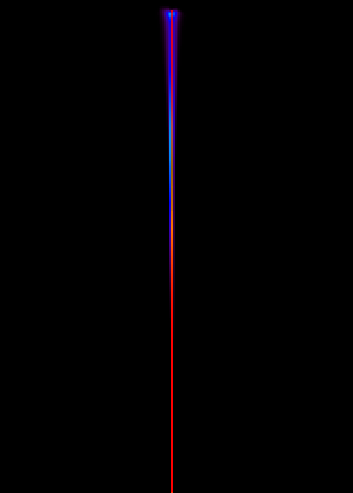
\includegraphics[width=0.49\textwidth, angle=90]{beam.png}
    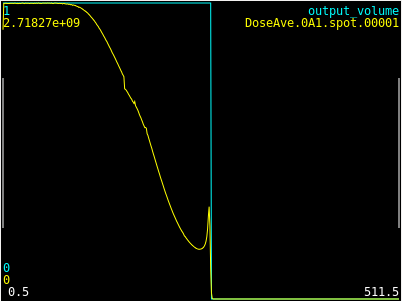
\includegraphics[width=0.49\textwidth]{profile.png}
    \caption{Beam with no $\sigma$ and $\epsilon$ in a patient (P15) and ray traced trajectory.}
\end{figure}

\section{Vector field probing}


\end{document}